% Created by tikzDevice version 0.12.6 on 2024-02-15 23:04:19
% !TEX encoding = UTF-8 Unicode
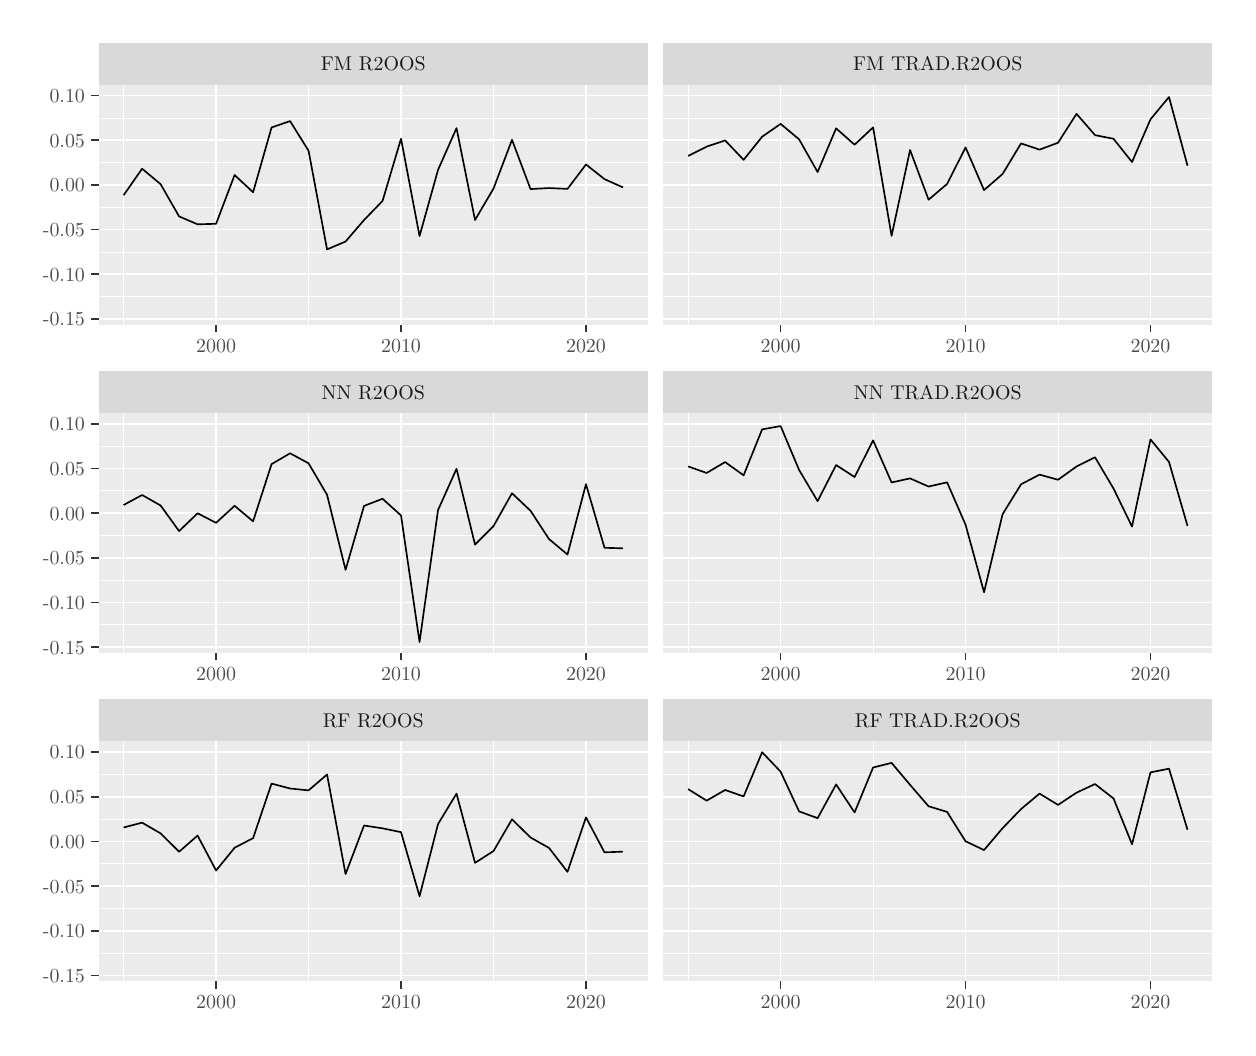
\begin{tikzpicture}[x=1pt,y=1pt]
\definecolor{fillColor}{RGB}{255,255,255}
\path[use as bounding box,fill=fillColor,fill opacity=0.00] (0,0) rectangle (433.62,361.35);
\begin{scope}
\path[clip] (  0.00,  0.00) rectangle (433.62,361.35);
\definecolor{drawColor}{RGB}{255,255,255}
\definecolor{fillColor}{RGB}{255,255,255}

\path[draw=drawColor,line width= 0.6pt,line join=round,line cap=round,fill=fillColor] (  0.00,  0.00) rectangle (433.62,361.35);
\end{scope}
\begin{scope}
\path[clip] ( 25.65,254.04) rectangle (224.13,340.69);
\definecolor{fillColor}{gray}{0.92}

\path[fill=fillColor] ( 25.65,254.04) rectangle (224.13,340.69);
\definecolor{drawColor}{RGB}{255,255,255}

\path[draw=drawColor,line width= 0.3pt,line join=round] ( 25.65,264.16) --
	(224.13,264.16);

\path[draw=drawColor,line width= 0.3pt,line join=round] ( 25.65,280.30) --
	(224.13,280.30);

\path[draw=drawColor,line width= 0.3pt,line join=round] ( 25.65,296.45) --
	(224.13,296.45);

\path[draw=drawColor,line width= 0.3pt,line join=round] ( 25.65,312.59) --
	(224.13,312.59);

\path[draw=drawColor,line width= 0.3pt,line join=round] ( 25.65,328.73) --
	(224.13,328.73);

\path[draw=drawColor,line width= 0.3pt,line join=round] ( 34.67,254.04) --
	( 34.67,340.69);

\path[draw=drawColor,line width= 0.3pt,line join=round] (101.50,254.04) --
	(101.50,340.69);

\path[draw=drawColor,line width= 0.3pt,line join=round] (168.33,254.04) --
	(168.33,340.69);

\path[draw=drawColor,line width= 0.6pt,line join=round] ( 25.65,256.08) --
	(224.13,256.08);

\path[draw=drawColor,line width= 0.6pt,line join=round] ( 25.65,272.23) --
	(224.13,272.23);

\path[draw=drawColor,line width= 0.6pt,line join=round] ( 25.65,288.37) --
	(224.13,288.37);

\path[draw=drawColor,line width= 0.6pt,line join=round] ( 25.65,304.52) --
	(224.13,304.52);

\path[draw=drawColor,line width= 0.6pt,line join=round] ( 25.65,320.66) --
	(224.13,320.66);

\path[draw=drawColor,line width= 0.6pt,line join=round] ( 25.65,336.81) --
	(224.13,336.81);

\path[draw=drawColor,line width= 0.6pt,line join=round] ( 68.08,254.04) --
	( 68.08,340.69);

\path[draw=drawColor,line width= 0.6pt,line join=round] (134.91,254.04) --
	(134.91,340.69);

\path[draw=drawColor,line width= 0.6pt,line join=round] (201.74,254.04) --
	(201.74,340.69);
\definecolor{drawColor}{RGB}{0,0,0}

\path[draw=drawColor,line width= 0.6pt,line join=round] ( 34.67,300.79) --
	( 41.35,310.38) --
	( 48.03,304.81) --
	( 54.72,293.14) --
	( 61.40,290.29) --
	( 68.08,290.48) --
	( 74.77,308.10) --
	( 81.45,301.87) --
	( 88.13,325.28) --
	( 94.82,327.59) --
	(101.50,316.87) --
	(108.18,281.23) --
	(114.87,284.07) --
	(121.55,291.84) --
	(128.23,298.73) --
	(134.91,321.21) --
	(141.60,286.05) --
	(148.28,309.95) --
	(154.96,325.05) --
	(161.65,291.86) --
	(168.33,303.21) --
	(175.01,320.82) --
	(181.70,303.03) --
	(188.38,303.39) --
	(195.06,303.09) --
	(201.74,311.91) --
	(208.43,306.62) --
	(215.11,303.63);
\end{scope}
\begin{scope}
\path[clip] ( 25.65,135.43) rectangle (224.13,222.07);
\definecolor{fillColor}{gray}{0.92}

\path[fill=fillColor] ( 25.65,135.43) rectangle (224.13,222.07);
\definecolor{drawColor}{RGB}{255,255,255}

\path[draw=drawColor,line width= 0.3pt,line join=round] ( 25.65,145.54) --
	(224.13,145.54);

\path[draw=drawColor,line width= 0.3pt,line join=round] ( 25.65,161.68) --
	(224.13,161.68);

\path[draw=drawColor,line width= 0.3pt,line join=round] ( 25.65,177.83) --
	(224.13,177.83);

\path[draw=drawColor,line width= 0.3pt,line join=round] ( 25.65,193.97) --
	(224.13,193.97);

\path[draw=drawColor,line width= 0.3pt,line join=round] ( 25.65,210.12) --
	(224.13,210.12);

\path[draw=drawColor,line width= 0.3pt,line join=round] ( 34.67,135.43) --
	( 34.67,222.07);

\path[draw=drawColor,line width= 0.3pt,line join=round] (101.50,135.43) --
	(101.50,222.07);

\path[draw=drawColor,line width= 0.3pt,line join=round] (168.33,135.43) --
	(168.33,222.07);

\path[draw=drawColor,line width= 0.6pt,line join=round] ( 25.65,137.47) --
	(224.13,137.47);

\path[draw=drawColor,line width= 0.6pt,line join=round] ( 25.65,153.61) --
	(224.13,153.61);

\path[draw=drawColor,line width= 0.6pt,line join=round] ( 25.65,169.76) --
	(224.13,169.76);

\path[draw=drawColor,line width= 0.6pt,line join=round] ( 25.65,185.90) --
	(224.13,185.90);

\path[draw=drawColor,line width= 0.6pt,line join=round] ( 25.65,202.05) --
	(224.13,202.05);

\path[draw=drawColor,line width= 0.6pt,line join=round] ( 25.65,218.19) --
	(224.13,218.19);

\path[draw=drawColor,line width= 0.6pt,line join=round] ( 68.08,135.43) --
	( 68.08,222.07);

\path[draw=drawColor,line width= 0.6pt,line join=round] (134.91,135.43) --
	(134.91,222.07);

\path[draw=drawColor,line width= 0.6pt,line join=round] (201.74,135.43) --
	(201.74,222.07);
\definecolor{drawColor}{RGB}{0,0,0}

\path[draw=drawColor,line width= 0.6pt,line join=round] ( 34.67,188.87) --
	( 41.35,192.48) --
	( 48.03,188.69) --
	( 54.72,179.44) --
	( 61.40,185.87) --
	( 68.08,182.42) --
	( 74.77,188.58) --
	( 81.45,182.96) --
	( 88.13,203.63) --
	( 94.82,207.55) --
	(101.50,203.93) --
	(108.18,192.55) --
	(114.87,165.42) --
	(121.55,188.53) --
	(128.23,191.12) --
	(134.91,185.08) --
	(141.60,139.36) --
	(148.28,187.03) --
	(154.96,201.95) --
	(161.65,174.54) --
	(168.33,181.25) --
	(175.01,193.11) --
	(181.70,186.78) --
	(188.38,176.56) --
	(195.06,170.97) --
	(201.74,196.40) --
	(208.43,173.41) --
	(215.11,173.20);
\end{scope}
\begin{scope}
\path[clip] ( 25.65, 16.81) rectangle (224.13,103.46);
\definecolor{fillColor}{gray}{0.92}

\path[fill=fillColor] ( 25.65, 16.81) rectangle (224.13,103.46);
\definecolor{drawColor}{RGB}{255,255,255}

\path[draw=drawColor,line width= 0.3pt,line join=round] ( 25.65, 26.92) --
	(224.13, 26.92);

\path[draw=drawColor,line width= 0.3pt,line join=round] ( 25.65, 43.07) --
	(224.13, 43.07);

\path[draw=drawColor,line width= 0.3pt,line join=round] ( 25.65, 59.21) --
	(224.13, 59.21);

\path[draw=drawColor,line width= 0.3pt,line join=round] ( 25.65, 75.36) --
	(224.13, 75.36);

\path[draw=drawColor,line width= 0.3pt,line join=round] ( 25.65, 91.50) --
	(224.13, 91.50);

\path[draw=drawColor,line width= 0.3pt,line join=round] ( 34.67, 16.81) --
	( 34.67,103.46);

\path[draw=drawColor,line width= 0.3pt,line join=round] (101.50, 16.81) --
	(101.50,103.46);

\path[draw=drawColor,line width= 0.3pt,line join=round] (168.33, 16.81) --
	(168.33,103.46);

\path[draw=drawColor,line width= 0.6pt,line join=round] ( 25.65, 18.85) --
	(224.13, 18.85);

\path[draw=drawColor,line width= 0.6pt,line join=round] ( 25.65, 35.00) --
	(224.13, 35.00);

\path[draw=drawColor,line width= 0.6pt,line join=round] ( 25.65, 51.14) --
	(224.13, 51.14);

\path[draw=drawColor,line width= 0.6pt,line join=round] ( 25.65, 67.28) --
	(224.13, 67.28);

\path[draw=drawColor,line width= 0.6pt,line join=round] ( 25.65, 83.43) --
	(224.13, 83.43);

\path[draw=drawColor,line width= 0.6pt,line join=round] ( 25.65, 99.57) --
	(224.13, 99.57);

\path[draw=drawColor,line width= 0.6pt,line join=round] ( 68.08, 16.81) --
	( 68.08,103.46);

\path[draw=drawColor,line width= 0.6pt,line join=round] (134.91, 16.81) --
	(134.91,103.46);

\path[draw=drawColor,line width= 0.6pt,line join=round] (201.74, 16.81) --
	(201.74,103.46);
\definecolor{drawColor}{RGB}{0,0,0}

\path[draw=drawColor,line width= 0.6pt,line join=round] ( 34.67, 72.34) --
	( 41.35, 74.08) --
	( 48.03, 70.21) --
	( 54.72, 63.58) --
	( 61.40, 69.41) --
	( 68.08, 56.79) --
	( 74.77, 65.01) --
	( 81.45, 68.49) --
	( 88.13, 88.20) --
	( 94.82, 86.42) --
	(101.50, 85.74) --
	(108.18, 91.48) --
	(114.87, 55.52) --
	(121.55, 73.06) --
	(128.23, 72.03) --
	(134.91, 70.65) --
	(141.60, 47.50) --
	(148.28, 73.57) --
	(154.96, 84.57) --
	(161.65, 59.55) --
	(168.33, 63.83) --
	(175.01, 75.29) --
	(181.70, 68.72) --
	(188.38, 64.96) --
	(195.06, 56.30) --
	(201.74, 75.99) --
	(208.43, 63.35) --
	(215.11, 63.61);
\end{scope}
\begin{scope}
\path[clip] (229.63,254.04) rectangle (428.12,340.69);
\definecolor{fillColor}{gray}{0.92}

\path[fill=fillColor] (229.63,254.04) rectangle (428.12,340.69);
\definecolor{drawColor}{RGB}{255,255,255}

\path[draw=drawColor,line width= 0.3pt,line join=round] (229.63,264.16) --
	(428.12,264.16);

\path[draw=drawColor,line width= 0.3pt,line join=round] (229.63,280.30) --
	(428.12,280.30);

\path[draw=drawColor,line width= 0.3pt,line join=round] (229.63,296.45) --
	(428.12,296.45);

\path[draw=drawColor,line width= 0.3pt,line join=round] (229.63,312.59) --
	(428.12,312.59);

\path[draw=drawColor,line width= 0.3pt,line join=round] (229.63,328.73) --
	(428.12,328.73);

\path[draw=drawColor,line width= 0.3pt,line join=round] (238.66,254.04) --
	(238.66,340.69);

\path[draw=drawColor,line width= 0.3pt,line join=round] (305.49,254.04) --
	(305.49,340.69);

\path[draw=drawColor,line width= 0.3pt,line join=round] (372.32,254.04) --
	(372.32,340.69);

\path[draw=drawColor,line width= 0.6pt,line join=round] (229.63,256.08) --
	(428.12,256.08);

\path[draw=drawColor,line width= 0.6pt,line join=round] (229.63,272.23) --
	(428.12,272.23);

\path[draw=drawColor,line width= 0.6pt,line join=round] (229.63,288.37) --
	(428.12,288.37);

\path[draw=drawColor,line width= 0.6pt,line join=round] (229.63,304.52) --
	(428.12,304.52);

\path[draw=drawColor,line width= 0.6pt,line join=round] (229.63,320.66) --
	(428.12,320.66);

\path[draw=drawColor,line width= 0.6pt,line join=round] (229.63,336.81) --
	(428.12,336.81);

\path[draw=drawColor,line width= 0.6pt,line join=round] (272.07,254.04) --
	(272.07,340.69);

\path[draw=drawColor,line width= 0.6pt,line join=round] (338.90,254.04) --
	(338.90,340.69);

\path[draw=drawColor,line width= 0.6pt,line join=round] (405.73,254.04) --
	(405.73,340.69);
\definecolor{drawColor}{RGB}{0,0,0}

\path[draw=drawColor,line width= 0.6pt,line join=round] (238.66,315.02) --
	(245.34,318.35) --
	(252.02,320.61) --
	(258.70,313.59) --
	(265.39,321.94) --
	(272.07,326.58) --
	(278.75,321.01) --
	(285.44,309.17) --
	(292.12,324.96) --
	(298.80,319.06) --
	(305.49,325.31) --
	(312.17,286.11) --
	(318.85,317.13) --
	(325.54,299.18) --
	(332.22,304.87) --
	(338.90,318.06) --
	(345.58,302.66) --
	(352.27,308.46) --
	(358.95,319.52) --
	(365.63,317.27) --
	(372.32,319.77) --
	(379.00,330.21) --
	(385.68,322.52) --
	(392.37,321.19) --
	(399.05,312.79) --
	(405.73,328.24) --
	(412.41,336.29) --
	(419.10,311.48);
\end{scope}
\begin{scope}
\path[clip] (229.63,135.43) rectangle (428.12,222.07);
\definecolor{fillColor}{gray}{0.92}

\path[fill=fillColor] (229.63,135.43) rectangle (428.12,222.07);
\definecolor{drawColor}{RGB}{255,255,255}

\path[draw=drawColor,line width= 0.3pt,line join=round] (229.63,145.54) --
	(428.12,145.54);

\path[draw=drawColor,line width= 0.3pt,line join=round] (229.63,161.68) --
	(428.12,161.68);

\path[draw=drawColor,line width= 0.3pt,line join=round] (229.63,177.83) --
	(428.12,177.83);

\path[draw=drawColor,line width= 0.3pt,line join=round] (229.63,193.97) --
	(428.12,193.97);

\path[draw=drawColor,line width= 0.3pt,line join=round] (229.63,210.12) --
	(428.12,210.12);

\path[draw=drawColor,line width= 0.3pt,line join=round] (238.66,135.43) --
	(238.66,222.07);

\path[draw=drawColor,line width= 0.3pt,line join=round] (305.49,135.43) --
	(305.49,222.07);

\path[draw=drawColor,line width= 0.3pt,line join=round] (372.32,135.43) --
	(372.32,222.07);

\path[draw=drawColor,line width= 0.6pt,line join=round] (229.63,137.47) --
	(428.12,137.47);

\path[draw=drawColor,line width= 0.6pt,line join=round] (229.63,153.61) --
	(428.12,153.61);

\path[draw=drawColor,line width= 0.6pt,line join=round] (229.63,169.76) --
	(428.12,169.76);

\path[draw=drawColor,line width= 0.6pt,line join=round] (229.63,185.90) --
	(428.12,185.90);

\path[draw=drawColor,line width= 0.6pt,line join=round] (229.63,202.05) --
	(428.12,202.05);

\path[draw=drawColor,line width= 0.6pt,line join=round] (229.63,218.19) --
	(428.12,218.19);

\path[draw=drawColor,line width= 0.6pt,line join=round] (272.07,135.43) --
	(272.07,222.07);

\path[draw=drawColor,line width= 0.6pt,line join=round] (338.90,135.43) --
	(338.90,222.07);

\path[draw=drawColor,line width= 0.6pt,line join=round] (405.73,135.43) --
	(405.73,222.07);
\definecolor{drawColor}{RGB}{0,0,0}

\path[draw=drawColor,line width= 0.6pt,line join=round] (238.66,202.80) --
	(245.34,200.44) --
	(252.02,204.38) --
	(258.70,199.59) --
	(265.39,216.19) --
	(272.07,217.39) --
	(278.75,201.53) --
	(285.44,190.27) --
	(292.12,203.30) --
	(298.80,198.98) --
	(305.49,212.21) --
	(312.17,197.01) --
	(318.85,198.48) --
	(325.54,195.54) --
	(332.22,197.05) --
	(338.90,181.75) --
	(345.58,157.34) --
	(352.27,185.52) --
	(358.95,196.34) --
	(365.63,199.84) --
	(372.32,197.98) --
	(379.00,202.78) --
	(385.68,206.12) --
	(392.37,194.80) --
	(399.05,181.07) --
	(405.73,212.56) --
	(412.41,204.43) --
	(419.10,181.33);
\end{scope}
\begin{scope}
\path[clip] (229.63, 16.81) rectangle (428.12,103.46);
\definecolor{fillColor}{gray}{0.92}

\path[fill=fillColor] (229.63, 16.81) rectangle (428.12,103.46);
\definecolor{drawColor}{RGB}{255,255,255}

\path[draw=drawColor,line width= 0.3pt,line join=round] (229.63, 26.92) --
	(428.12, 26.92);

\path[draw=drawColor,line width= 0.3pt,line join=round] (229.63, 43.07) --
	(428.12, 43.07);

\path[draw=drawColor,line width= 0.3pt,line join=round] (229.63, 59.21) --
	(428.12, 59.21);

\path[draw=drawColor,line width= 0.3pt,line join=round] (229.63, 75.36) --
	(428.12, 75.36);

\path[draw=drawColor,line width= 0.3pt,line join=round] (229.63, 91.50) --
	(428.12, 91.50);

\path[draw=drawColor,line width= 0.3pt,line join=round] (238.66, 16.81) --
	(238.66,103.46);

\path[draw=drawColor,line width= 0.3pt,line join=round] (305.49, 16.81) --
	(305.49,103.46);

\path[draw=drawColor,line width= 0.3pt,line join=round] (372.32, 16.81) --
	(372.32,103.46);

\path[draw=drawColor,line width= 0.6pt,line join=round] (229.63, 18.85) --
	(428.12, 18.85);

\path[draw=drawColor,line width= 0.6pt,line join=round] (229.63, 35.00) --
	(428.12, 35.00);

\path[draw=drawColor,line width= 0.6pt,line join=round] (229.63, 51.14) --
	(428.12, 51.14);

\path[draw=drawColor,line width= 0.6pt,line join=round] (229.63, 67.28) --
	(428.12, 67.28);

\path[draw=drawColor,line width= 0.6pt,line join=round] (229.63, 83.43) --
	(428.12, 83.43);

\path[draw=drawColor,line width= 0.6pt,line join=round] (229.63, 99.57) --
	(428.12, 99.57);

\path[draw=drawColor,line width= 0.6pt,line join=round] (272.07, 16.81) --
	(272.07,103.46);

\path[draw=drawColor,line width= 0.6pt,line join=round] (338.90, 16.81) --
	(338.90,103.46);

\path[draw=drawColor,line width= 0.6pt,line join=round] (405.73, 16.81) --
	(405.73,103.46);
\definecolor{drawColor}{RGB}{0,0,0}

\path[draw=drawColor,line width= 0.6pt,line join=round] (238.66, 86.19) --
	(245.34, 82.03) --
	(252.02, 85.89) --
	(258.70, 83.56) --
	(265.39, 99.52) --
	(272.07, 92.51) --
	(278.75, 78.15) --
	(285.44, 75.71) --
	(292.12, 87.88) --
	(298.80, 77.78) --
	(305.49, 94.01) --
	(312.17, 95.68) --
	(318.85, 87.74) --
	(325.54, 80.00) --
	(332.22, 77.97) --
	(338.90, 67.36) --
	(345.58, 64.18) --
	(352.27, 72.08) --
	(358.95, 78.98) --
	(365.63, 84.58) --
	(372.32, 80.50) --
	(379.00, 84.92) --
	(385.68, 88.03) --
	(392.37, 82.82) --
	(399.05, 66.28) --
	(405.73, 92.25) --
	(412.41, 93.59) --
	(419.10, 71.52);
\end{scope}
\begin{scope}
\path[clip] ( 25.65,103.46) rectangle (224.13,118.62);
\definecolor{fillColor}{gray}{0.85}

\path[fill=fillColor] ( 25.65,103.46) rectangle (224.13,118.62);
\definecolor{drawColor}{gray}{0.10}

\node[text=drawColor,anchor=base,inner sep=0pt, outer sep=0pt, scale=  0.72] at (124.89,108.56) {RF R2OOS};
\end{scope}
\begin{scope}
\path[clip] (229.63,103.46) rectangle (428.12,118.62);
\definecolor{fillColor}{gray}{0.85}

\path[fill=fillColor] (229.63,103.46) rectangle (428.12,118.62);
\definecolor{drawColor}{gray}{0.10}

\node[text=drawColor,anchor=base,inner sep=0pt, outer sep=0pt, scale=  0.72] at (328.88,108.56) {RF TRAD.R2OOS};
\end{scope}
\begin{scope}
\path[clip] ( 25.65,222.07) rectangle (224.13,237.23);
\definecolor{fillColor}{gray}{0.85}

\path[fill=fillColor] ( 25.65,222.07) rectangle (224.13,237.23);
\definecolor{drawColor}{gray}{0.10}

\node[text=drawColor,anchor=base,inner sep=0pt, outer sep=0pt, scale=  0.72] at (124.89,227.17) {NN R2OOS};
\end{scope}
\begin{scope}
\path[clip] (229.63,222.07) rectangle (428.12,237.23);
\definecolor{fillColor}{gray}{0.85}

\path[fill=fillColor] (229.63,222.07) rectangle (428.12,237.23);
\definecolor{drawColor}{gray}{0.10}

\node[text=drawColor,anchor=base,inner sep=0pt, outer sep=0pt, scale=  0.72] at (328.88,227.17) {NN TRAD.R2OOS};
\end{scope}
\begin{scope}
\path[clip] ( 25.65,340.69) rectangle (224.13,355.85);
\definecolor{fillColor}{gray}{0.85}

\path[fill=fillColor] ( 25.65,340.69) rectangle (224.13,355.85);
\definecolor{drawColor}{gray}{0.10}

\node[text=drawColor,anchor=base,inner sep=0pt, outer sep=0pt, scale=  0.72] at (124.89,345.79) {FM R2OOS};
\end{scope}
\begin{scope}
\path[clip] (229.63,340.69) rectangle (428.12,355.85);
\definecolor{fillColor}{gray}{0.85}

\path[fill=fillColor] (229.63,340.69) rectangle (428.12,355.85);
\definecolor{drawColor}{gray}{0.10}

\node[text=drawColor,anchor=base,inner sep=0pt, outer sep=0pt, scale=  0.72] at (328.88,345.79) {FM TRAD.R2OOS};
\end{scope}
\begin{scope}
\path[clip] (  0.00,  0.00) rectangle (433.62,361.35);
\definecolor{drawColor}{gray}{0.20}

\path[draw=drawColor,line width= 0.6pt,line join=round] ( 68.08, 14.06) --
	( 68.08, 16.81);

\path[draw=drawColor,line width= 0.6pt,line join=round] (134.91, 14.06) --
	(134.91, 16.81);

\path[draw=drawColor,line width= 0.6pt,line join=round] (201.74, 14.06) --
	(201.74, 16.81);
\end{scope}
\begin{scope}
\path[clip] (  0.00,  0.00) rectangle (433.62,361.35);
\definecolor{drawColor}{gray}{0.30}

\node[text=drawColor,anchor=base,inner sep=0pt, outer sep=0pt, scale=  0.72] at ( 68.08,  6.90) {2000};

\node[text=drawColor,anchor=base,inner sep=0pt, outer sep=0pt, scale=  0.72] at (134.91,  6.90) {2010};

\node[text=drawColor,anchor=base,inner sep=0pt, outer sep=0pt, scale=  0.72] at (201.74,  6.90) {2020};
\end{scope}
\begin{scope}
\path[clip] (  0.00,  0.00) rectangle (433.62,361.35);
\definecolor{drawColor}{gray}{0.20}

\path[draw=drawColor,line width= 0.6pt,line join=round] (272.07, 14.06) --
	(272.07, 16.81);

\path[draw=drawColor,line width= 0.6pt,line join=round] (338.90, 14.06) --
	(338.90, 16.81);

\path[draw=drawColor,line width= 0.6pt,line join=round] (405.73, 14.06) --
	(405.73, 16.81);
\end{scope}
\begin{scope}
\path[clip] (  0.00,  0.00) rectangle (433.62,361.35);
\definecolor{drawColor}{gray}{0.30}

\node[text=drawColor,anchor=base,inner sep=0pt, outer sep=0pt, scale=  0.72] at (272.07,  6.90) {2000};

\node[text=drawColor,anchor=base,inner sep=0pt, outer sep=0pt, scale=  0.72] at (338.90,  6.90) {2010};

\node[text=drawColor,anchor=base,inner sep=0pt, outer sep=0pt, scale=  0.72] at (405.73,  6.90) {2020};
\end{scope}
\begin{scope}
\path[clip] (  0.00,  0.00) rectangle (433.62,361.35);
\definecolor{drawColor}{gray}{0.20}

\path[draw=drawColor,line width= 0.6pt,line join=round] ( 68.08,132.68) --
	( 68.08,135.43);

\path[draw=drawColor,line width= 0.6pt,line join=round] (134.91,132.68) --
	(134.91,135.43);

\path[draw=drawColor,line width= 0.6pt,line join=round] (201.74,132.68) --
	(201.74,135.43);
\end{scope}
\begin{scope}
\path[clip] (  0.00,  0.00) rectangle (433.62,361.35);
\definecolor{drawColor}{gray}{0.30}

\node[text=drawColor,anchor=base,inner sep=0pt, outer sep=0pt, scale=  0.72] at ( 68.08,125.52) {2000};

\node[text=drawColor,anchor=base,inner sep=0pt, outer sep=0pt, scale=  0.72] at (134.91,125.52) {2010};

\node[text=drawColor,anchor=base,inner sep=0pt, outer sep=0pt, scale=  0.72] at (201.74,125.52) {2020};
\end{scope}
\begin{scope}
\path[clip] (  0.00,  0.00) rectangle (433.62,361.35);
\definecolor{drawColor}{gray}{0.20}

\path[draw=drawColor,line width= 0.6pt,line join=round] (272.07,132.68) --
	(272.07,135.43);

\path[draw=drawColor,line width= 0.6pt,line join=round] (338.90,132.68) --
	(338.90,135.43);

\path[draw=drawColor,line width= 0.6pt,line join=round] (405.73,132.68) --
	(405.73,135.43);
\end{scope}
\begin{scope}
\path[clip] (  0.00,  0.00) rectangle (433.62,361.35);
\definecolor{drawColor}{gray}{0.30}

\node[text=drawColor,anchor=base,inner sep=0pt, outer sep=0pt, scale=  0.72] at (272.07,125.52) {2000};

\node[text=drawColor,anchor=base,inner sep=0pt, outer sep=0pt, scale=  0.72] at (338.90,125.52) {2010};

\node[text=drawColor,anchor=base,inner sep=0pt, outer sep=0pt, scale=  0.72] at (405.73,125.52) {2020};
\end{scope}
\begin{scope}
\path[clip] (  0.00,  0.00) rectangle (433.62,361.35);
\definecolor{drawColor}{gray}{0.20}

\path[draw=drawColor,line width= 0.6pt,line join=round] ( 68.08,251.29) --
	( 68.08,254.04);

\path[draw=drawColor,line width= 0.6pt,line join=round] (134.91,251.29) --
	(134.91,254.04);

\path[draw=drawColor,line width= 0.6pt,line join=round] (201.74,251.29) --
	(201.74,254.04);
\end{scope}
\begin{scope}
\path[clip] (  0.00,  0.00) rectangle (433.62,361.35);
\definecolor{drawColor}{gray}{0.30}

\node[text=drawColor,anchor=base,inner sep=0pt, outer sep=0pt, scale=  0.72] at ( 68.08,244.13) {2000};

\node[text=drawColor,anchor=base,inner sep=0pt, outer sep=0pt, scale=  0.72] at (134.91,244.13) {2010};

\node[text=drawColor,anchor=base,inner sep=0pt, outer sep=0pt, scale=  0.72] at (201.74,244.13) {2020};
\end{scope}
\begin{scope}
\path[clip] (  0.00,  0.00) rectangle (433.62,361.35);
\definecolor{drawColor}{gray}{0.20}

\path[draw=drawColor,line width= 0.6pt,line join=round] (272.07,251.29) --
	(272.07,254.04);

\path[draw=drawColor,line width= 0.6pt,line join=round] (338.90,251.29) --
	(338.90,254.04);

\path[draw=drawColor,line width= 0.6pt,line join=round] (405.73,251.29) --
	(405.73,254.04);
\end{scope}
\begin{scope}
\path[clip] (  0.00,  0.00) rectangle (433.62,361.35);
\definecolor{drawColor}{gray}{0.30}

\node[text=drawColor,anchor=base,inner sep=0pt, outer sep=0pt, scale=  0.72] at (272.07,244.13) {2000};

\node[text=drawColor,anchor=base,inner sep=0pt, outer sep=0pt, scale=  0.72] at (338.90,244.13) {2010};

\node[text=drawColor,anchor=base,inner sep=0pt, outer sep=0pt, scale=  0.72] at (405.73,244.13) {2020};
\end{scope}
\begin{scope}
\path[clip] (  0.00,  0.00) rectangle (433.62,361.35);
\definecolor{drawColor}{gray}{0.30}

\node[text=drawColor,anchor=base east,inner sep=0pt, outer sep=0pt, scale=  0.72] at ( 20.70,253.61) {-0.15};

\node[text=drawColor,anchor=base east,inner sep=0pt, outer sep=0pt, scale=  0.72] at ( 20.70,269.75) {-0.10};

\node[text=drawColor,anchor=base east,inner sep=0pt, outer sep=0pt, scale=  0.72] at ( 20.70,285.89) {-0.05};

\node[text=drawColor,anchor=base east,inner sep=0pt, outer sep=0pt, scale=  0.72] at ( 20.70,302.04) {0.00};

\node[text=drawColor,anchor=base east,inner sep=0pt, outer sep=0pt, scale=  0.72] at ( 20.70,318.18) {0.05};

\node[text=drawColor,anchor=base east,inner sep=0pt, outer sep=0pt, scale=  0.72] at ( 20.70,334.33) {0.10};
\end{scope}
\begin{scope}
\path[clip] (  0.00,  0.00) rectangle (433.62,361.35);
\definecolor{drawColor}{gray}{0.20}

\path[draw=drawColor,line width= 0.6pt,line join=round] ( 22.90,256.08) --
	( 25.65,256.08);

\path[draw=drawColor,line width= 0.6pt,line join=round] ( 22.90,272.23) --
	( 25.65,272.23);

\path[draw=drawColor,line width= 0.6pt,line join=round] ( 22.90,288.37) --
	( 25.65,288.37);

\path[draw=drawColor,line width= 0.6pt,line join=round] ( 22.90,304.52) --
	( 25.65,304.52);

\path[draw=drawColor,line width= 0.6pt,line join=round] ( 22.90,320.66) --
	( 25.65,320.66);

\path[draw=drawColor,line width= 0.6pt,line join=round] ( 22.90,336.81) --
	( 25.65,336.81);
\end{scope}
\begin{scope}
\path[clip] (  0.00,  0.00) rectangle (433.62,361.35);
\definecolor{drawColor}{gray}{0.30}

\node[text=drawColor,anchor=base east,inner sep=0pt, outer sep=0pt, scale=  0.72] at ( 20.70,134.99) {-0.15};

\node[text=drawColor,anchor=base east,inner sep=0pt, outer sep=0pt, scale=  0.72] at ( 20.70,151.13) {-0.10};

\node[text=drawColor,anchor=base east,inner sep=0pt, outer sep=0pt, scale=  0.72] at ( 20.70,167.28) {-0.05};

\node[text=drawColor,anchor=base east,inner sep=0pt, outer sep=0pt, scale=  0.72] at ( 20.70,183.42) {0.00};

\node[text=drawColor,anchor=base east,inner sep=0pt, outer sep=0pt, scale=  0.72] at ( 20.70,199.57) {0.05};

\node[text=drawColor,anchor=base east,inner sep=0pt, outer sep=0pt, scale=  0.72] at ( 20.70,215.71) {0.10};
\end{scope}
\begin{scope}
\path[clip] (  0.00,  0.00) rectangle (433.62,361.35);
\definecolor{drawColor}{gray}{0.20}

\path[draw=drawColor,line width= 0.6pt,line join=round] ( 22.90,137.47) --
	( 25.65,137.47);

\path[draw=drawColor,line width= 0.6pt,line join=round] ( 22.90,153.61) --
	( 25.65,153.61);

\path[draw=drawColor,line width= 0.6pt,line join=round] ( 22.90,169.76) --
	( 25.65,169.76);

\path[draw=drawColor,line width= 0.6pt,line join=round] ( 22.90,185.90) --
	( 25.65,185.90);

\path[draw=drawColor,line width= 0.6pt,line join=round] ( 22.90,202.05) --
	( 25.65,202.05);

\path[draw=drawColor,line width= 0.6pt,line join=round] ( 22.90,218.19) --
	( 25.65,218.19);
\end{scope}
\begin{scope}
\path[clip] (  0.00,  0.00) rectangle (433.62,361.35);
\definecolor{drawColor}{gray}{0.30}

\node[text=drawColor,anchor=base east,inner sep=0pt, outer sep=0pt, scale=  0.72] at ( 20.70, 16.37) {-0.15};

\node[text=drawColor,anchor=base east,inner sep=0pt, outer sep=0pt, scale=  0.72] at ( 20.70, 32.52) {-0.10};

\node[text=drawColor,anchor=base east,inner sep=0pt, outer sep=0pt, scale=  0.72] at ( 20.70, 48.66) {-0.05};

\node[text=drawColor,anchor=base east,inner sep=0pt, outer sep=0pt, scale=  0.72] at ( 20.70, 64.81) {0.00};

\node[text=drawColor,anchor=base east,inner sep=0pt, outer sep=0pt, scale=  0.72] at ( 20.70, 80.95) {0.05};

\node[text=drawColor,anchor=base east,inner sep=0pt, outer sep=0pt, scale=  0.72] at ( 20.70, 97.09) {0.10};
\end{scope}
\begin{scope}
\path[clip] (  0.00,  0.00) rectangle (433.62,361.35);
\definecolor{drawColor}{gray}{0.20}

\path[draw=drawColor,line width= 0.6pt,line join=round] ( 22.90, 18.85) --
	( 25.65, 18.85);

\path[draw=drawColor,line width= 0.6pt,line join=round] ( 22.90, 35.00) --
	( 25.65, 35.00);

\path[draw=drawColor,line width= 0.6pt,line join=round] ( 22.90, 51.14) --
	( 25.65, 51.14);

\path[draw=drawColor,line width= 0.6pt,line join=round] ( 22.90, 67.28) --
	( 25.65, 67.28);

\path[draw=drawColor,line width= 0.6pt,line join=round] ( 22.90, 83.43) --
	( 25.65, 83.43);

\path[draw=drawColor,line width= 0.6pt,line join=round] ( 22.90, 99.57) --
	( 25.65, 99.57);
\end{scope}
\end{tikzpicture}
